Esta sección se realizará la máquina de \acrlong{htb} llamada \textit{Cap}\cite{cap}. \textit{Cap} es una máquina de dificultad ``fácil``.

\subsection{Reconocimiento}
En la fase de reconocimiento hemos encontrado la información de la máquina en la propia página principal\cite{cap} de la misma. Se ha encontrado que es una máquina \textit{Linux} y que su IP es \texttt{10.10.10.245}.

Dado que es un \acrshort{CTF}, no se ha visto la necesidad de indagar más en esta fase.

\subsection{Enumeración}
El primer paso realizado en la enumeración es usar la herramienta \textit{Nmap}\cite{nmap}. Para ello se ha utilizado el siguiente comando.
\begin{lstlisting}[language=bash]
nmap -p- --min-rate 10000 -o ports.txt 10.10.10.245
\end{lstlisting}
El argumento \texttt{-p-} para hacer un escaneo de todos los puertos; \texttt{--min-rate 10000} se ha utilizado para indicar a \textit{Nmap} que como mínimo envíe 10000 paquetes por segundo; por último, el argumento \texttt{-o ports.txt}, que es utilizado para guardar la salida en un archivo llamado ports.txt.

Tras la ejecución del comando, se han encontrado los puertos 21/\acrshort{tcp}, 22/\acrshort{tcp} y 80/\acrshort{tcp} abiertos. Con este resultado, de nuevo ejecutamos \textit{Nmap} para sacar información sobre los servicios que se están ejecutando en cada puerto.

Se ha utilizado el siguiente comando:
\begin{lstlisting}[language=bash]
sudo nmap -p 21,22,80 -sS -sCV 10.10.10.245 -o nmap.txt
\end{lstlisting}

Esta vez, el comando \texttt{-p} recibe los puertos obtenidos con el comando anterior, es decir, los puertos 21, 22 y 80 \acrshort{tcp}. Se ha decidido hacer un escaneo de tipo \textit{Stealth}, ya que es la manera más rápida y popular para escanear en el protocolo TCP; para ello se ha utilizado el argumento \texttt{-sS}. Se ha utilizado el comando \texttt{-sCV} para obtener información sobre el servicio habilitado en el puerto (\texttt{-sV}) y para realizar el escaneo con los scripts por defecto de \textit{Nmap} (\texttt{-sC}). Por último, también se ha decidido guardar la salida del comando en un archivo (argumento \texttt{-o} llamado nmap.txt.

Tras la ejecución se ha encontrado que, efectivamente, la máquina es un sistema \textit{Linux}, concretamente con el sistema operativo \textit{Ubuntu}. Como era de esperar, en el puerto 21/\acrshort{tcp} se ha encontrado un servidor \acrshort{ftp}, está corriendo \textit{vsftpd}\cite{vsftpd} en la versión 3.0.3. En el puerto 22/\acrshort{tcp} está levantado un servidor \acrshort{ssh}, está utilizando \textit{OpenSSH}\cite{openssh} versión 8.2p1. Por último, en el puerto 80/\acrshort{tcp} un servidor \acrshort{http} \textit{Gunicorn}\cite{gunicorn}.

En este fase, también se ha decidido utilizar la herramienta \textit{Gobuster}\cite{gobuster} en la web, para encontrar endpoints no accesibles a primera vista. Para ello, se ha utilizado el siguiente comando:
\begin{lstlisting}[language=bash]
gobuster dir -u http://10.10.10.245 -w ~/Hacking/SecLists/Discovery/Web-Content/raft-large-directories.txt | anew gobuster.txt
\end{lstlisting}
Se ha elegido el argumento \texttt{dir} para realizar una búsquedad de directorios mediante fuerza bruta; el flag \texttt{-u} es el utilizado para pasar la \acrshort{url} que vamos  a escanear; el argumento \texttt{-w} se utiliza para pasarle a \textit{Gobuster} una lista de palabras para utilizar. En este caso se ha decidido usar la lista \textit{raft-large-directories.txt} de \textit{SecLists}\cite{seclists}. Por último, el resultado de \textit{Gobuster} se ha decidido pasar a la herrameinta \textit{anew}\cite{anew} porque también se ha realizado el mismo comando pero con la lista \textit{raft-large-words.txt}.

Como resultado se han encontrado las siguientes \acrshort{url}'s:
\begin{itemize}
    \item \texttt{/}
    \item \texttt{/data}
    \item \texttt{/ip}
    \item \texttt{/capture} (redirecciona a \texttt{/data})
    \item \texttt{/netstat}
\end{itemize}

\subsection{Ganar acceso}

Lo primero que se ha intentado es acceder al servicio \acrshort{ssh} con contraseñas débiles, como \textit{admin:admin}, \textit{admin:Passw0rd} o \textit{admin:123456}, pero ninguna ha dado resultado.

Acto seguido se ha decidido investigar la web. Al abrir la página web \texttt{http://10.10.10.245}, lo primero que encontramos es un dashboard (figura \ref{fig:cap-dashboard}). Vemos que ya estamos logeados como \textit{Nathan}, y que algunos de los botones no funcionan, como \textit{Message} y \textit{Settings}.
\begin{figure}[h]
    \centering
    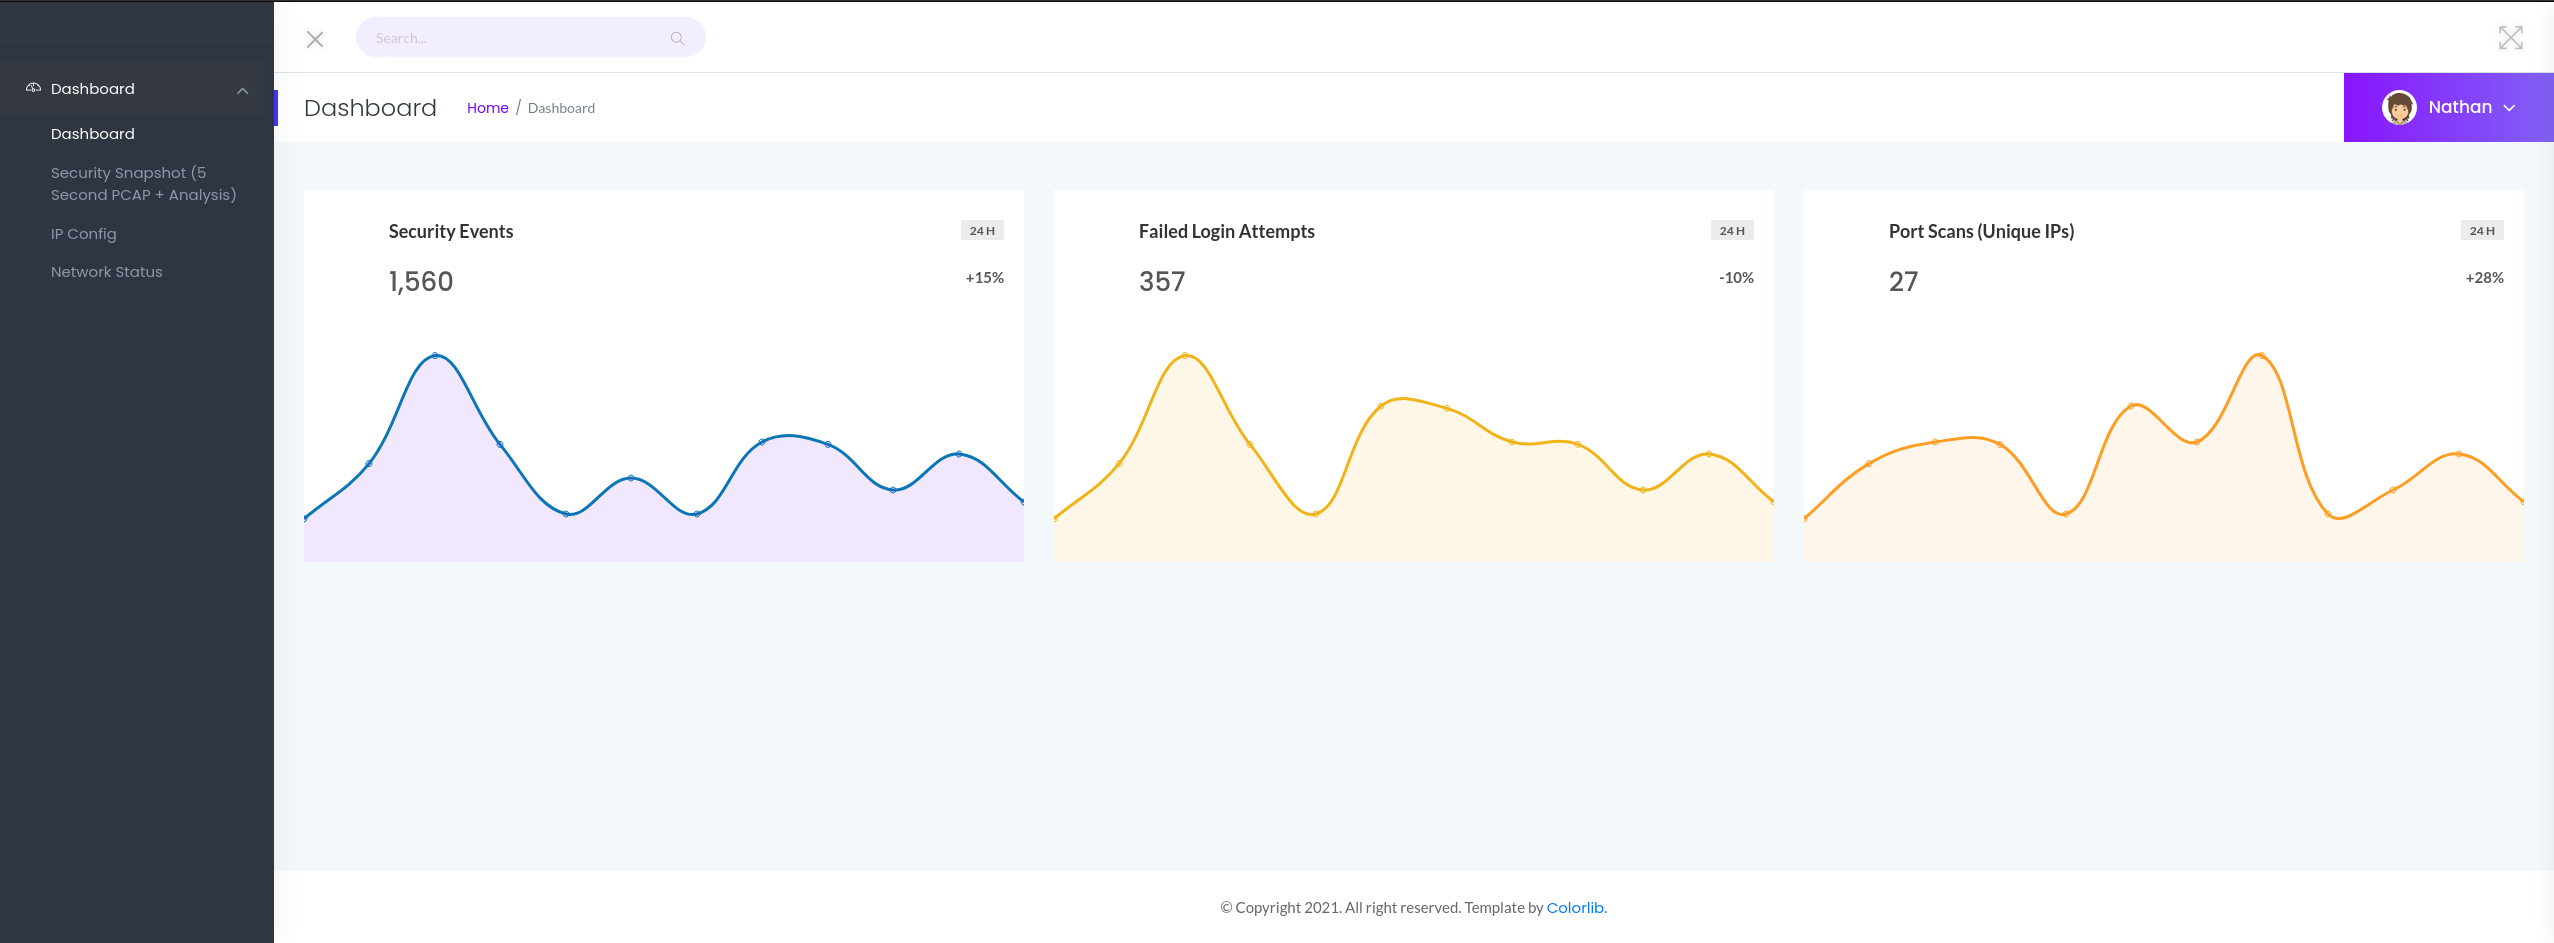
\includegraphics[width=1.0\textwidth]{images/machines/cap/web-dashboard.png}
    \caption{Cap: Dashboard (\texttt{http://10.10.10.245})}
    \label{fig:cap-dashboard}
\end{figure}

También se ha investigado las pestañas del menú lateral izquierdo. Encontramos información de la red en los apartados \textit{IP Config} (figura \ref{fig:cap-net}-a) y \textit{Network Status} (figura \ref{fig:cap-net}-b).

\begin{figure}
    \centering
    \subfloat[\centering \textit{Cap: IP Config (\texttt{http://10.10.10.245/ip})}]{{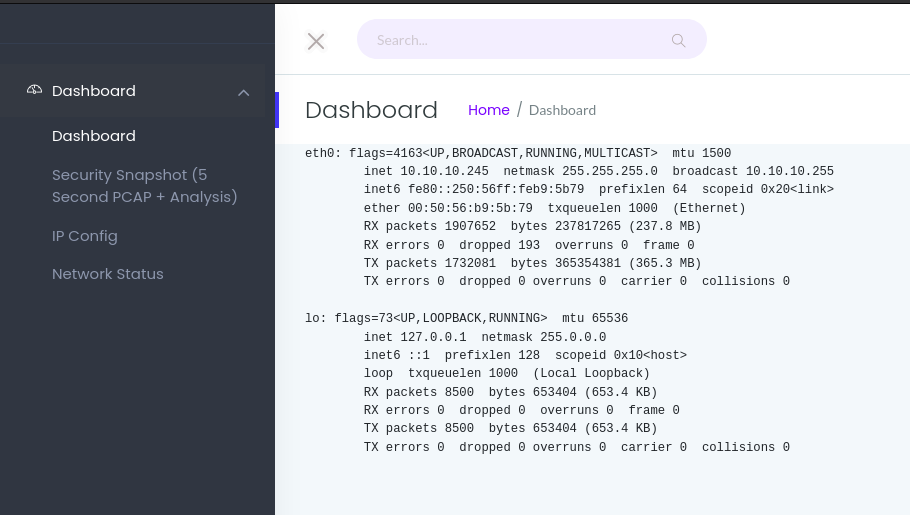
\includegraphics[width=0.70\textwidth]{images/machines/cap/web-ip.png} }}%
    \qquad
    \subfloat[\centering \textit{Cap: Network Status (\texttt{http://10.10.10.245/netstat})}]{{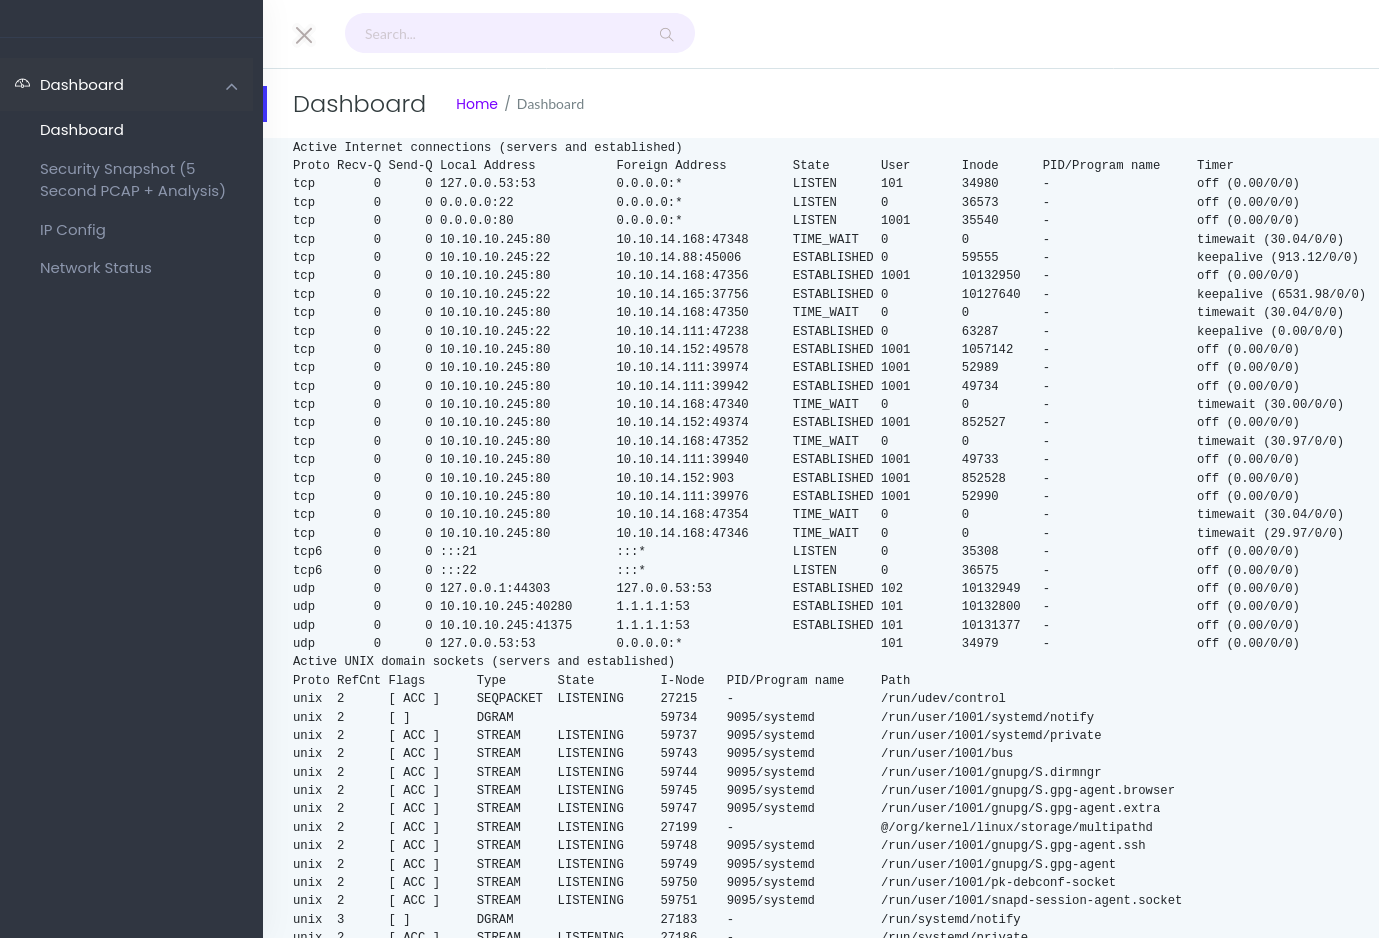
\includegraphics[width=0.75\textwidth]{images/machines/cap/web-network.png} }}
    \caption{Cap Información de red}
    \label{fig:cap-net}
\end{figure}

Por último, el apartado Security Snapshot (figura \ref{fig:cap-snapshot}) nos permite descargar un paquete \texttt{.pcap}.

\begin{figure}[h]
    \centering
    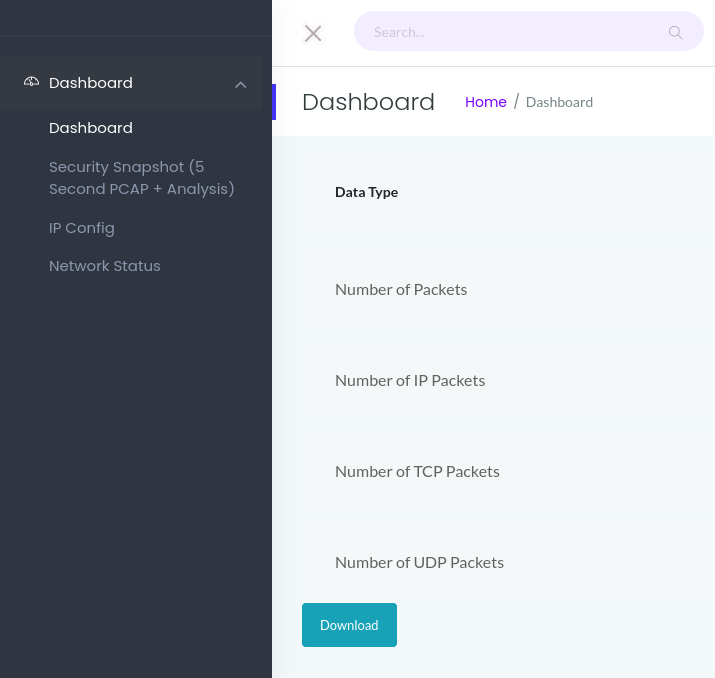
\includegraphics[width=0.40\textwidth]{images/machines/cap/web-sec-snapshots.png}
    \caption{Cap: Security Snapshot (\texttt{http://10.10.10.245/data/16})}
    \label{fig:cap-snapshot}
\end{figure}

Al clicar el botón \textit{Download}, nos bajamos un archivo llamado \textit{16.pcap}. Nombre que coincide con la \acrshort{url}, ya que esta es \texttt{/data/16}. Investigamos el paquete con \textit{Wireshark}\cite{wireshark} (figura \ref{fig:cap-wire-16})

\begin{figure}[h]
    \centering
    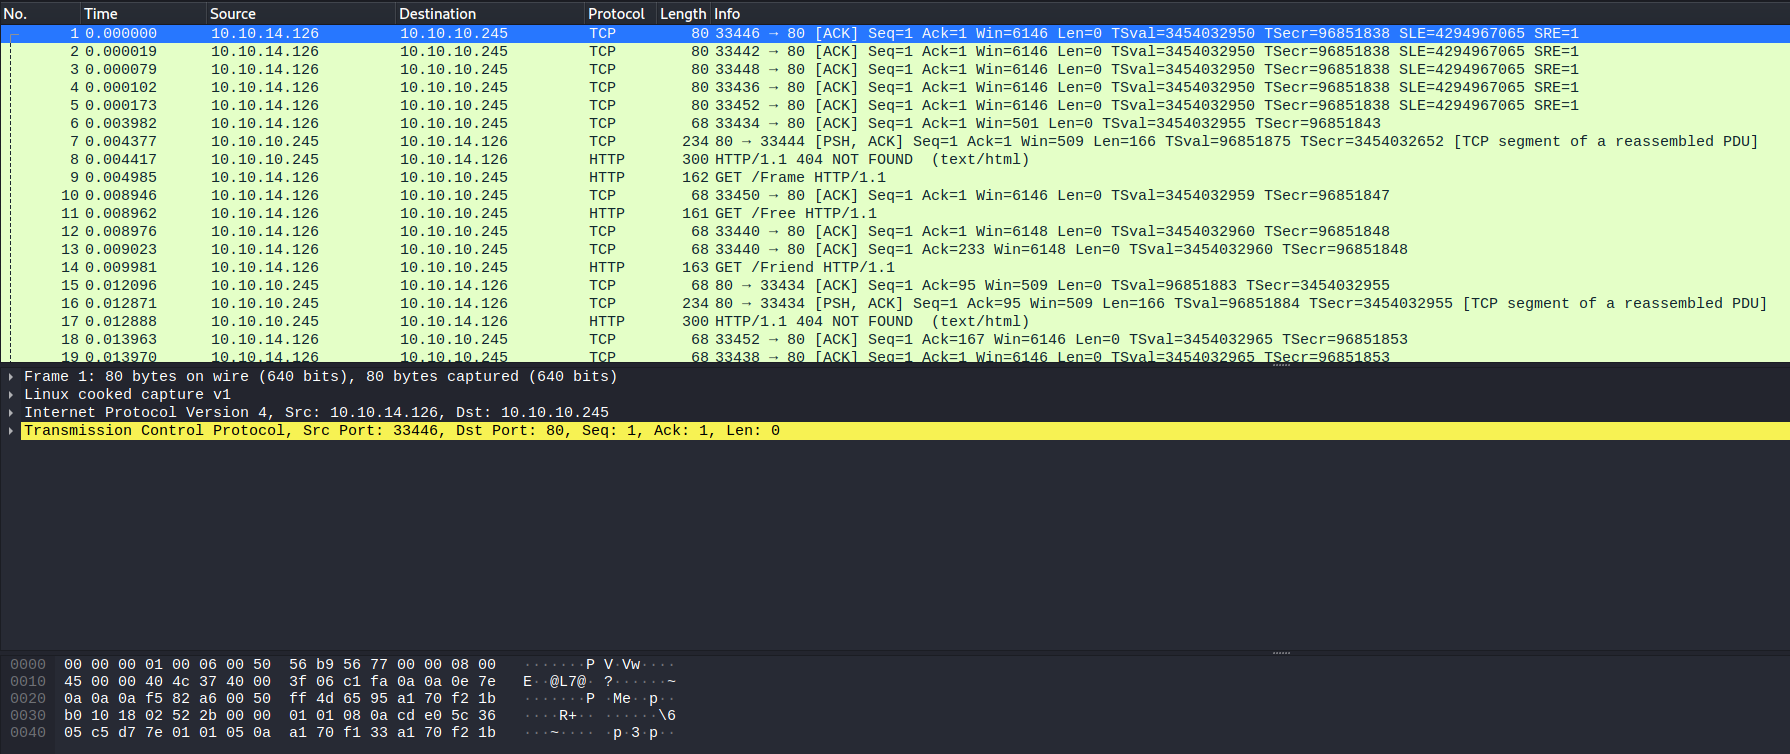
\includegraphics[width=1.0\textwidth]{images/machines/cap/wireshark-16.png}
    \caption{Archivo \textit{16.pcap} en \textit{Wireshark}}
    \label{fig:cap-wire-16}
\end{figure}

Tras investigar los paquetes, no se ha encontrado nada relevante. Tampoco se ha encontrado nada sobre los servicios \acrshort{ssh} y \acrshort{ftp}.\\

Al no encontrar nada en este paquete, se ha decidido probar con la \acrshort{url} \texttt{/data/\{?\}}. Se ha probado con los valores `0`, `1` y `1000`. En los casos `0` y `1` hemos conseguido entrar a \texttt{/data/0} y \texttt{/data/1} descargar los paquetes \texttt{0.pcap} y \texttt{1.pcap}, pero con el valor `1000` hemos sido redirigidos a la página principal.\\

Se ha decidido empezar por orden, y empezar revisando primero \texttt{0.pcap}. Al revisar el paquete, encontramos que en este hay movimiento en los puertos 21 y 22. Además, encontramos un inicio de sesión exitoso en el servidor \acrshort{ftp}. Como se ve en la figura \ref{fig:cap-wire-0}, se encuentran las credenciales \textit{nathan:Buck3tH4TF0RM3!}.
\begin{figure}[h]
    \centering
    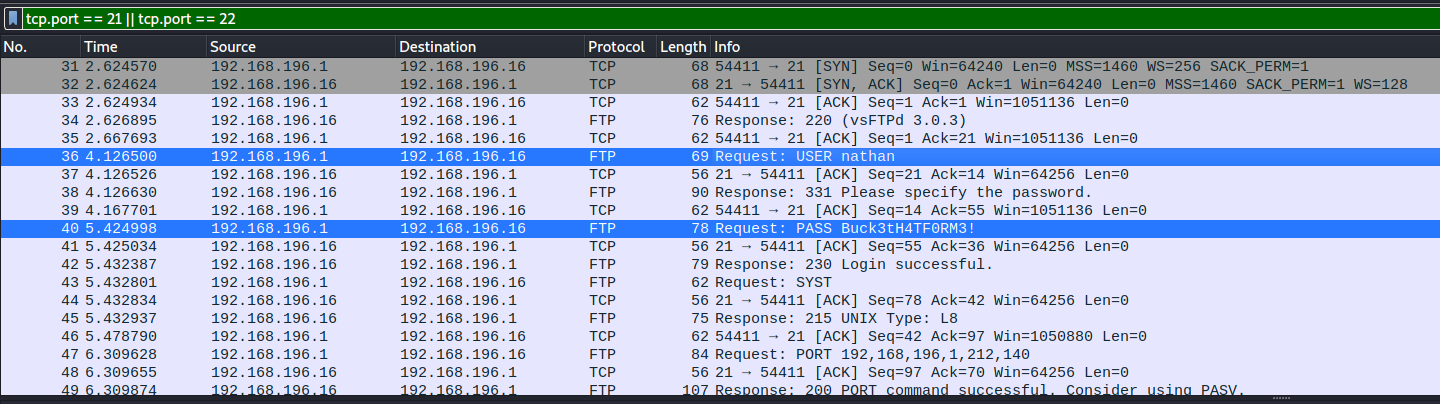
\includegraphics[width=1.0\textwidth]{images/machines/cap/wireshark-0.png}
    \caption{Archivo \textit{0.pcap} en \textit{Wireshark}}
    \label{fig:cap-wire-0}
\end{figure}

Con las credenciales obtenidas, entramos al servidor \acrshort{ftp}, y, como se ve en la figura \ref{fig:cap-user-flag}, obtenemos el flag de usuario.
\begin{figure}[h]
    \centering
    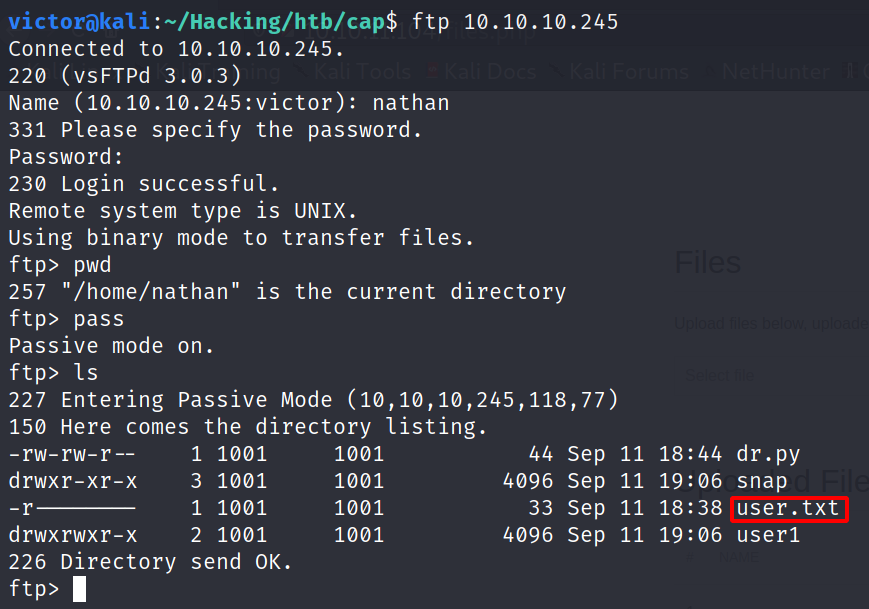
\includegraphics[width=0.8\textwidth]{images/machines/cap/user-flag.png}
    \caption{Acceso al servidor \acrshort{ftp} y obtención del flag de usuario}
    \label{fig:cap-user-flag}
\end{figure}

\subsection{Escalada de Privilegios}

Lo primero que se decide hacer es intentar acceder al \acrshort{ssh} con las credenciales anteriores. Conseguimos entrar.\\

Primero, intentamos ver si el usuario \textit{nathan} puede ejecutar algo como súper-usuario. Vemos que \textit{nathan} no puede usar \texttt{sudo} (figura \ref{fig:cap-nathan-sudo}).

\begin{figure}[h]
    \centering
    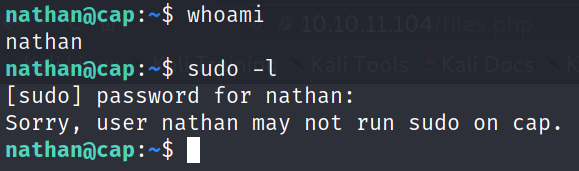
\includegraphics[width=0.5\textwidth]{images/machines/cap/nathan-sudo.png}
    \caption{Login \acrshort{ssh} con \textit{nathan} y comprobación de \texttt{sudo}}
    \label{fig:cap-nathan-sudo}
\end{figure}

Para encontrar si el usuario \textit{nathan} puede ejecutar algún comando con permisos de súper-usuario, se ha utilizado la herramienta \textit{linPEAS}\cite{peas}. Para poder utilizar \textit{linPEAS}, tenemos que tener el script en la máquina víctima. Para pasar el script de nuestro host a la máquina, se ha utilizado el siguiente comando:
\begin{lstlisting}[language=bash]
scp ./linpeas.sh nathan@10.10.10.245:/home/nathan
\end{lstlisting}

Una vez subido el script, lo ejecutamos con:
\begin{lstlisting}[language=bash]
./linpeas.sh
\end{lstlisting}

Y como resultado vemos que \textit{nathan} puede utilizar \texttt{/usr/bin/python3.8} como \textit{root} (figura \ref{fig:cap-linpeas}).\\

\begin{figure}[h]
    \centering
    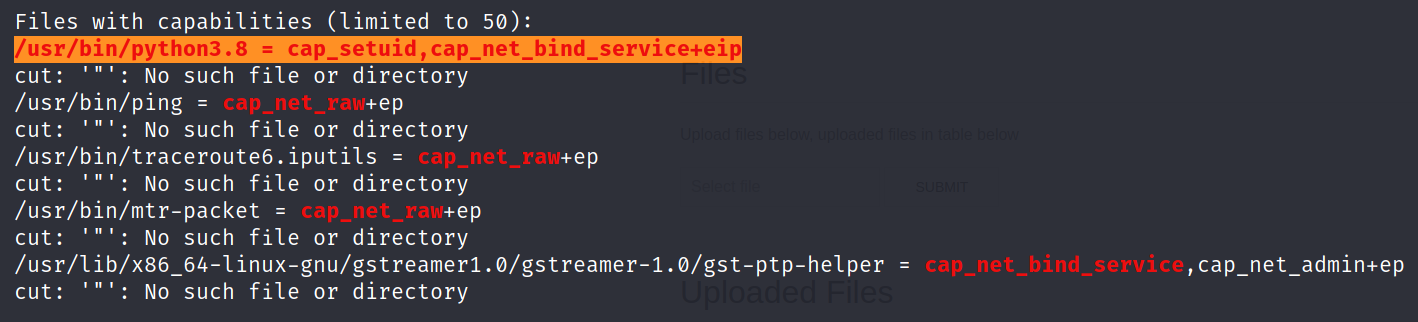
\includegraphics[width=1.0\textwidth]{images/machines/cap/linpeas.png}
    \caption{Resultado \textit{linPEAS}}
    \label{fig:cap-linpeas}
\end{figure}

Se ha investigado sobre posibles payloads y al final se ha decidido usar el siguiente para ganar acceso como \textit{root} (figura \ref{fig:cap-root}).
\begin{lstlisting}[language=bash]
python3 -c "import os; os.setuid(0); os.system('/bin/bash -i')"
\end{lstlisting}

\begin{figure}[h]
    \centering
    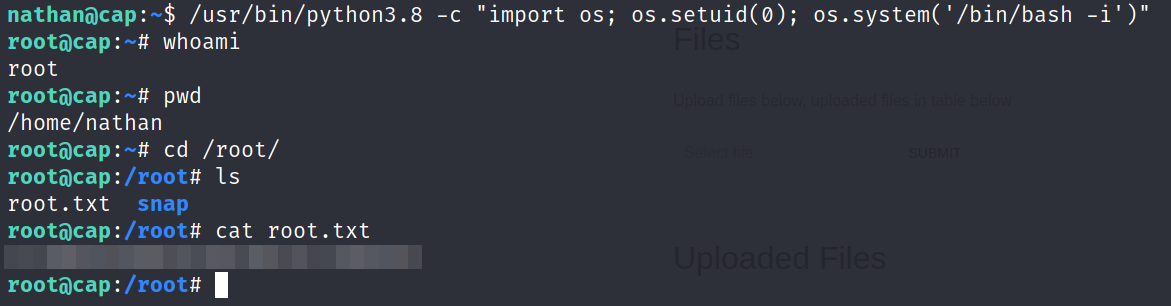
\includegraphics[width=0.7\textwidth]{images/machines/cap/root.png}
    \caption{Escalada de privilegios y obtención de \textit{root}}
    \label{fig:cap-root}
\end{figure}
